\documentclass{article}
\usepackage[utf8x]{inputenc}
\usepackage{ucs}
\usepackage{amsmath} 
\usepackage{amsfonts}
\usepackage{marvosym}
\usepackage{wasysym}
\usepackage{upgreek}
\usepackage[english,russian]{babel}
\usepackage{graphicx}
\usepackage{float}
\usepackage{textcomp}
\usepackage{hyperref}
\usepackage{geometry}
  \geometry{left=2cm}
  \geometry{right=1.5cm}
  \geometry{top=1cm}
  \geometry{bottom=2cm}
\usepackage{tikz}
\usepackage{ccaption}
\usepackage{multicol}

\hypersetup{
   colorlinks=true,
   citecolor=blue,
   linkcolor=black,
   urlcolor=blue
}

\usepackage{listings}
%\setlength{\columnsep}{1.5cm}
%\setlength{\columnseprule}{0.2pt}

\usepackage[absolute]{textpos}

\usepackage{colortbl,graphicx,tikz}
\definecolor{X}{rgb}{.5,.5,.5}


\begin{document}
\pagenumbering{gobble}
\lstset{
  language=C,                % choose the language of the code
  basicstyle=\linespread{1.1}\ttfamily,
  columns=fixed,
  fontadjust=true,
  basewidth=0.5em,
  keywordstyle=\color{blue}\bfseries,
  commentstyle=\color{gray},
  stringstyle=\ttfamily\color{orange!50!black},
  showstringspaces=false,
  numbersep=5pt,
  numberstyle=\tiny\color{black},
  numberfirstline=true,
  stepnumber=1,                   % the step between two line-numbers.        
  numbersep=10pt,                  % how far the line-numbers are from the code
  backgroundcolor=\color{white},  % choose the background color. You must add \usepackage{color}
  showstringspaces=false,         % underline spaces within strings
  captionpos=b,                   % sets the caption-position to bottom
  breaklines=true,                % sets automatic line breaking
  breakatwhitespace=true,         % sets if automatic breaks should only happen at whitespace
  xleftmargin=.2in,
  extendedchars=\true,
  keepspaces = true,
}
\lstset{literate=%
   *{0}{{{\color{red!20!violet}0}}}1
    {1}{{{\color{red!20!violet}1}}}1
    {2}{{{\color{red!20!violet}2}}}1
    {3}{{{\color{red!20!violet}3}}}1
    {4}{{{\color{red!20!violet}4}}}1
    {5}{{{\color{red!20!violet}5}}}1
    {6}{{{\color{red!20!violet}6}}}1
    {7}{{{\color{red!20!violet}7}}}1
    {8}{{{\color{red!20!violet}8}}}1
    {9}{{{\color{red!20!violet}9}}}1
}

\title{Семинар \#9: Сортировки. Домашнее задание.\vspace{-5ex}}\date{}\maketitle

\section*{Сложность алгоритмов}
\subsubsection*{Чему равна средняя вычислительная сложность следующих операций?}
\begin{enumerate}
\item Поиск элемента в неотсортированном массиве размера $N$
\item Поиск элемента в отсортированном массиве размера $N$ (бинарный поиск)
\item Добавление элемента в начало массива размера $N$
\item Добавление элемента в конец массива размера $N$ (в предположении, что \texttt{capacity} > \texttt{size})
\item Добавление элемента в динамический(саморасширяющийся) стек размера $N$  при аддитивной стратегии выделения памяти (при нехватки места увеличиваем \texttt{capacity} на некоторую постоянную величину).
\item Добавление элемента в динамический стек размера $N$ при мультипликативной стратегии выделения памяти (при нехватки места умножаем \texttt{capacity} на некоторую постоянную величину (обычно на 2)).
\item Сортировка выбором массива размера $N$
\item Сортировка пузырьком массива размера $N$
\item Быстрая сортировка массива размера $N$
\item Сортировка подсчётом массива размера $N$, если максимальный элемент массива равен $K$
\item Цифровая сортировка массива размера $N$, если максимальный элемент массива равен $K$
\item Сортировка Bogosort массива размера $N$
\item Сложение двух чисел длиной в $N$ цифр ($N$ может быть большим)
\item Простой алгоритм умножения(столбиком) двух чисел длиной в $N$ цифр ($N$ может быть большим)
\item Простой алгоритм проверки числа на простоту перебором от двух до корня этого числа. Число состоит из $N$ цифр в десятичной записи ($N$ может быть большим)
\item $\!\!\!\!{^*}$ Добавление элемента в двоичную кучу размера $N$
\item $\!\!\!\!{^*}$ Удаление элемента из двоичной кучи размера $N$
\end{enumerate}
Нужно написать ответы в текстовый файл и прислать мне.
\newpage
\section*{Быстрая сортировка - Quicksort}
\begin{multicols}{2}
\begin{lstlisting}
#include <stdio.h>
#include <stdlib.h>
#define N 30

void quicksort(int* array, int lo, int hi)
{
    if (hi - lo > 1)
    {
        int j = lo;
        int pivot = array[hi - 1];
        for (int i = lo; i < hi; i++)
            if (array[i] <= pivot)
            {
                int temp = array[i];
                array[i] = array[j];
                array[j] = temp;
                j++;
            }

        quicksort(array, lo, j - 1);
        quicksort(array, j, hi);
    }
}

void print(int* array, int n)
{
    for (int i = 0; i < n; i++)
        printf("%d ", array[i]);
    printf("\n");
}

int main()
{
    int numbers[N];
    for(int i = 0; i < N; i++)
        numbers[i] = rand() % 100;
    
    print(numbers, N);
    quicksort(numbers, 0, N);
    print(numbers, N);
}
\end{lstlisting}
\vfill\null
\columnbreak
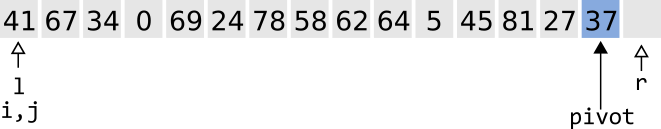
\includegraphics[scale=0.53]{../images/qs2.png}
\\
\\
\\
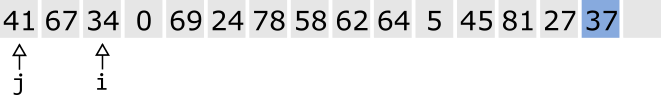
\includegraphics[scale=0.53]{../images/qs4.png}
\\
\\
\\
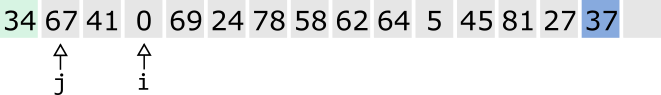
\includegraphics[scale=0.53]{../images/qs5.png}
\\
\\
\\
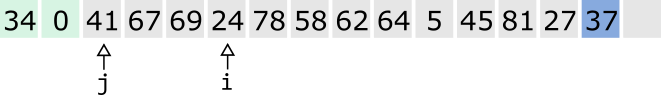
\includegraphics[scale=0.53]{../images/qs6.png}
\\
\\
\\
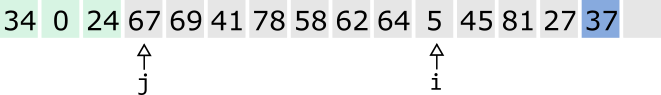
\includegraphics[scale=0.53]{../images/qs7.png}
\\
\\
\\
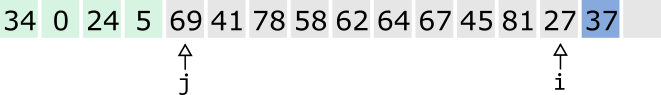
\includegraphics[scale=0.53]{../images/qs8.png}
\\
\\
\\
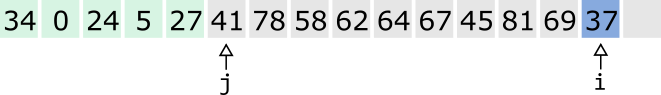
\includegraphics[scale=0.53]{../images/qs9.png}
\\
\\
\\
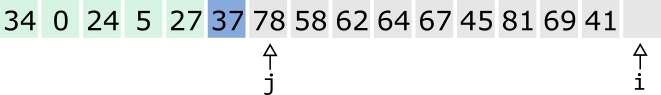
\includegraphics[scale=0.53]{../images/qs10.png}
\\
\\
\\
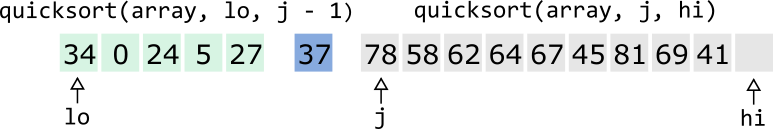
\includegraphics[scale=0.47]{../images/qs11.png}
\end{multicols}
\newpage
\textbf{Задача: Звёзды:} В файле \texttt{hipstars.csv} содержится информация о ближайших звёздах. Данные взяты из каталога Hipparcos. В каждой строке - информация об одной звезде:
\begin{enumerate}
\item \texttt{hip} - номер звезды в каталоге Hipparcos. Обратите внимание, что не все звёзды из каталога присутствуют в файле.
\item \texttt{proper\_name} - традиционное имя звезды(строка не более чем 20 символов). Большинство звёзд имён не имеют и называются просто по номеру, например HIP 3345. Если у звезды имени нет, то в этом поле стоит прочерк \texttt{-\,-}.
\item \texttt{right\_ascension} и \texttt{declination} - прямое восхождение и склонение определяют положение звезды на небе. Аналог широты и долготы. (\texttt{double})
\item \texttt{magnitude} - Звёздная величина - яркость звезды с точки зрения земного наблюдателя. Чем меньше, тем звезда ярче, шкала логарифмическая. Видимые глазом звёзды имеют звёздную величину 6 и ниже. Бетельгейзе $= 0.45$ Сириус $= -1.44$. Луна $= -12.7$. Солнце $= -26.7$.  (\texttt{float})
\item \texttt{absolute\_magnitude} Абсолютная звёздная величина - яркость звезды с точки зрения наблюдателя, находящегося на растоянии в 10 парсек от этой звезды. Бетельгейзе $= -5.47$. Сириус $= 1.45$. Солнце $= 4.85$. (\texttt{float})
\item \texttt{spectral\_type} - спектральный класс звезды(2 символа). 
\item \texttt{x}, \texttt{y} и \texttt{z} - Координаты звёзды в системе отсчёта, связанной с Землёй. Единица измерения - парсеки. \\
$1$ парсек = $3.26$ световых года = $206265$ расстояний от Земли до Солнца = $3 \cdot 10^{16}$ метров. (\texttt{float})
\item \texttt{constellation} - Созвездие (первые три буквы) или \texttt{NO}, если звезда не входит ни в какое созвездие.
\end{enumerate}
\begin{itemize}
\item Опишите структуру \texttt{Star}, которая будет предназначена для хранения информации об одной звезде.
\item \textbf{Считываем звёзды:}\\ 
Формат \texttt{.csv} (comma-separated values) -- это простейший формат для хранения табличных данных. В первой строке этого формата содержатся имена колонок таблицы, разделённые запятыми. Дальше -- \texttt{n} строк таблицы, все величины в таблице разделены запятыми. Эти файлы можно открывать как в обычном текстовом редакторе, так и в программах для работы с таблицами (например, Excel). Если файл \texttt{hipstars.csv} открыть в текстовом редакторе, то его начало будет выглядеть примерно так:
\begin{verbatim}
hip,proper_name,ra,dec,mag,absmag,spectral_type,x,y,z,constellation
0,Sol,0.00000,0.00000,-26.70,4.85,G2,0.000005,0.000,0.000,NO
1,--,0.00090,1.08901,9.10,2.39,F5,219.741,0.003,4.177,Psc
2,--,0.00424,-19.49884,9.27,5.87,K3,45.211,0.003,-16.009,Cet
3,--,0.00503,38.85928,6.61,-1.62,B9,344.553,0.030,277.615,And
4,--,0.00853,-51.89355,8.06,2.42,F0,82.836,0.012,-105.620,Phe
\end{verbatim}
Для считывания используйте функцию \texttt{fscanf} из библиотеки \texttt{stdio.h}. Учтите, что спецификатор \texttt{\%s} считывает строку до пробела. Чтобы считать строку до запятой используйте спецификатор \texttt{\%[\textasciicircum,]} - при этом \texttt{s} на конец спецификатора ставить не надо. Пример считывания:
\begin{lstlisting}
#include <stdio.h>

int main()
{
    // Открываем файл hipstars.csv на чтение("r").
    FILE* f = fopen("hipstars.csv", "r");
    // Считываем первую строку
    char header[200];
    fscanf(f, "%s\n", header);
    // Считываем звезду
    fscanf(f, "%d,%[^,],%lf,%lf,%f,%f,%[^,],%f,%f,%f,%[^\n]\n", ...)
    // ...
    fclose(f);
}
\end{lstlisting}

Создайте массив из структур \texttt{Star} подходящего размера и считайте все данные из файла в массив. Файл содержит информацию о $114318$ звезде, так что массив нужно создавать в куче (с помощью \texttt{malloc}). \\

\item \textbf{Сохраняем звёзды:}\\ Написать функцию \texttt{void save\_stars(char* filename, char* header, Star* array, int n)}, которая будет сохранять звёзды из массива \texttt{array} в файл, чьё название хранится в переменной \texttt{filename}. Например, при вызове \texttt{save\_stars(``output.csv'', header, stars, n);} массив \texttt{stars} должен сохраниться в файл \texttt{output.csv}. Первая строка в этом файле будет являться строкой \texttt{header}, в которой хранится название колонок.

\item \textbf{Сортировка по видимой с Земли яркости:}\\ Создайте функцию \texttt{quicksort\_magnitude}, чтобы она принимала на вход массив из структур \texttt{Star} и сортировала их по возрастанию звёздной величины. Проверьте функцию в \texttt{main}, отсортировав структуры и сохранив их в файл \texttt{sorted\_by\_magnitude.csv} с помощью функции \texttt{save\_stars}.

\item \textbf{Сортировка по расстоянию:}\\ Создайте функцию \texttt{quicksort\_distance}, чтобы она сортировала массив звёзд по расстоянию от Земли. Проверьте функцию в \texttt{main}, отсортировав структуры и сохранив их в файл \texttt{sorted\_by\_distance.csv}.

\item \textbf{Сортировка по температуре:}\\ Создайте функцию \texttt{quicksort\_temperature}, чтобы она сортировала массив звёзд по температуре поверхности. Темературу можно сравнить по первым двум символам спектра. Первый символ - спектральный класс звезды - от горячих к холодным: \texttt{O->B->A->F->G->K->M}. Второй символ - подкласс - число от 0 до 9, чем меньше, тем горячее. То есть теоретически самые горячие звёзды это звёзды класса \texttt{A0}, а самые холодные это звёзды класса \texttt{M9}. Проверьте функцию в \texttt{main}, отсортировав структуры и сохранив их в файл \texttt{sorted\_by\_temperature.csv}.\\
Сложность этой задачи в том, что может быть много звёзд с одинаковым спектральным классом. Предположим, что подмассив для сортировки оказался тривиальным и все его элементы оказались равны друг другу. В этом случае наша \texttt{quicksort} не будет делить массив на 2 части (все элементы будут равны \texttt{pivot} и окажутся слева). В таком случае наша \texttt{quicksort} будет работать очень медленно. Чтобы этого избежать, вам нужно будет видоизменить функцию \texttt{quicksort} так, чтобы она делила массив на 3 части (элементы меньшие \texttt{pivot}, равные \texttt{pivot} и большие \texttt{pivot}) и продолжала сортировать только первую и третью части.

\item \textbf{Функция-компаратор:}\\ Объедините три предыдущие функции в одну с использованием функции-компаратора. Нужно написать функцию \texttt{void quicksort(Star* array, int lo, int hi, int (*cmp)(Star* a, Star* b))}, которая будет сортировать звёзды, основываясь на функции-компараторе \texttt{cmp}. \\
Функция-компаратор принимает 2 указателя на элементы массива и возвращает:
\begin{itemize}
\item положительное число, если \texttt{*b} должен идти в отсортированом массиве правее \texttt{*a}.
\item отрицательное число, если \texttt{*b} должен идти в отсортированом массиве левее \texttt{*a}.
\item \texttt{0}, если нужно сохранить текущий порядок элементов.
\end{itemize} 


\end{itemize}

Эта задача очень похожа на задачу сортировки городов из классных задач. Решение можете посмотреть в папке \texttt{cities}. Там есть 2 программы: \texttt{sort\_cities.c} -- сортирует города и \texttt{sort\_cities\_funcpointer.c} -- сортирует города с использованием функции компаратора.

\newpage
\section*{Сегменты памяти. Указатели на функцию.}
\begin{multicols}{2}
\begin{center}
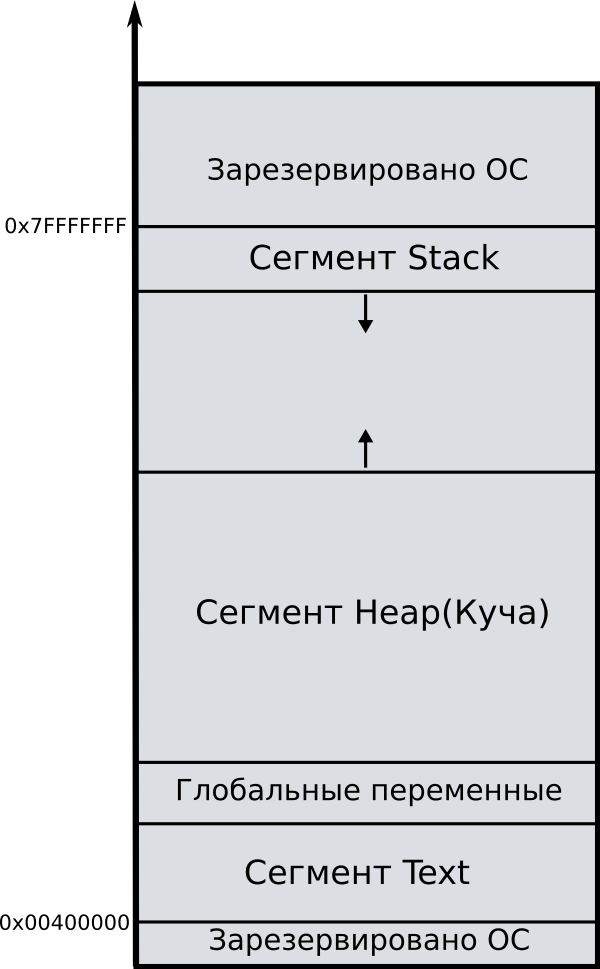
\includegraphics[scale=1.4]{../images/memory_layout.png}
\end{center}
\columnbreak
\begin{enumerate}
\item \textbf{Сегмент памяти Стек (Stack)} \\
\begin{itemize}
\item При обычном объявлении переменных и массивов все они создаются в стеке: \texttt{int a;} или \texttt{int array[10];}
\item Память на эти переменные выделяется в начале функции и освобождается в конце функции.
\item Маленький размер (несколько мегабайт)
\item Выделение памяти происходит быстрее чем в куче
\end{itemize}
\item \textbf{Сегмент памяти Куча (Heap)} \\
\begin{itemize}
\item \texttt{malloc} выделяет память в Куче. \\
\texttt{int* p = (int*)malloc(10 * sizeof(int));}
\item Память выделяется при вызове \texttt{malloc} и освобождается при вызове \texttt{free}.
\item Размер ограничен свободной оперативной памятью - гигабайты.
\item Выделение памяти происходит медленней чем в стеке
\end{itemize}
\item \textbf{Сегмент памяти Text} \\
\begin{itemize}
\item В этом сегменте хранится машинный код программы (Код на языке C, сначала, переводится в код на языке Ассемблера, а потом в машинный код. Как это происходит смотрите ниже.).
\item Адрес функции - адрес первого байта инструкций в этом сегменте.
\end{itemize}
\end{enumerate}
\end{multicols}

Пример работы с указателем на функцию:
\begin{lstlisting}
#include <stdio.h>

void print(int a)
{
    printf("%d\n", a);
}
int main ()
{
    // Создадим указатель на функцию ( вместо названия функции - *p )
    void (*p)(int a) = print;
    
    // Теперь с p можно работать также как и с print
    p(123);
}
\end{lstlisting}
Подробней в файле \texttt{funcpointers/0funcpointer.c}.
\newpage
\textbf{Задачи на указатели на функцию:}
\begin{itemize}
\item В файле \texttt{funcpointers/1foreach.c} лежит заготовка исходного кода. Вам нужно написать функцию\\ \texttt{void foreach(int* array, int size, int (*f)(int))}, которая будет принимать на вход массив размера \texttt{size} и применять к каждому элементу функцию \texttt{f}.

\item В файле \texttt{funcpointers/2foreach\_second\_argument.c} лежит заготовка исходного кода. Вам нужно написать функцию\\ \texttt{void foreach(int* array, int size, int (*f)(int, int), int b)}, которая будет принимать на вход массив размера \texttt{size} и применять к каждому элементу функцию \texttt{g(x) = f(x, b)}.
\end{itemize}


\section*{Стандартная функция qsort}

В библиотеке \texttt{stdlib.h} уже реализована функция \texttt{qsort}, которая сортирует произвольные элементы, используя быструю сортировку. Пример использования этой функции:
\begin{lstlisting}
#include <stdio.h>
#include <stdlib.h>

int cmp(const void* a, const void* b)
{
    // В этот компаратор передаются указатели на void,
    // Поэтому их нужно привести в нужный нам тип:
    int* pa = (int*)a;
    int* pb = (int*)b;
    return (*pa - *pb);
}

int main()
{
    int arr[] = {163, 624, 7345, 545, 41, 78, 5, 536, 962, 1579};
    qsort(arr, 10, sizeof(int), cmp);
    // qsort( массив, количество элементов, размер каждого элемента, компаратор )
    // Функция принимает на вход указатель на функцию cmp
   
    print_array(10, arr);
}
\end{lstlisting}
Функция-компаратор стандартной функции \texttt{qsort} отличается от той, что была написана нами для сортировки
городов и звёзд только тем, что она принимает на вход указатели типа \texttt{void*}. Это сделано для того, чтобы эта функция была более общей. С помощью неё можно отсортировать как массив чисел, так и массив указателей или массив любых структур. В функции \texttt{cmp} нужно привести указатель \texttt{void*} к указателю нужного типа.\\
\textbf{Задача на стандартную функцию \texttt{qsort}:}
\begin{itemize}
\item Перепишите сортировку звёзд с использованием функции \texttt{qsort}.
\end{itemize}
\newpage
\subsection*{Как код превращается в последовательность байт:}
\begin{center}
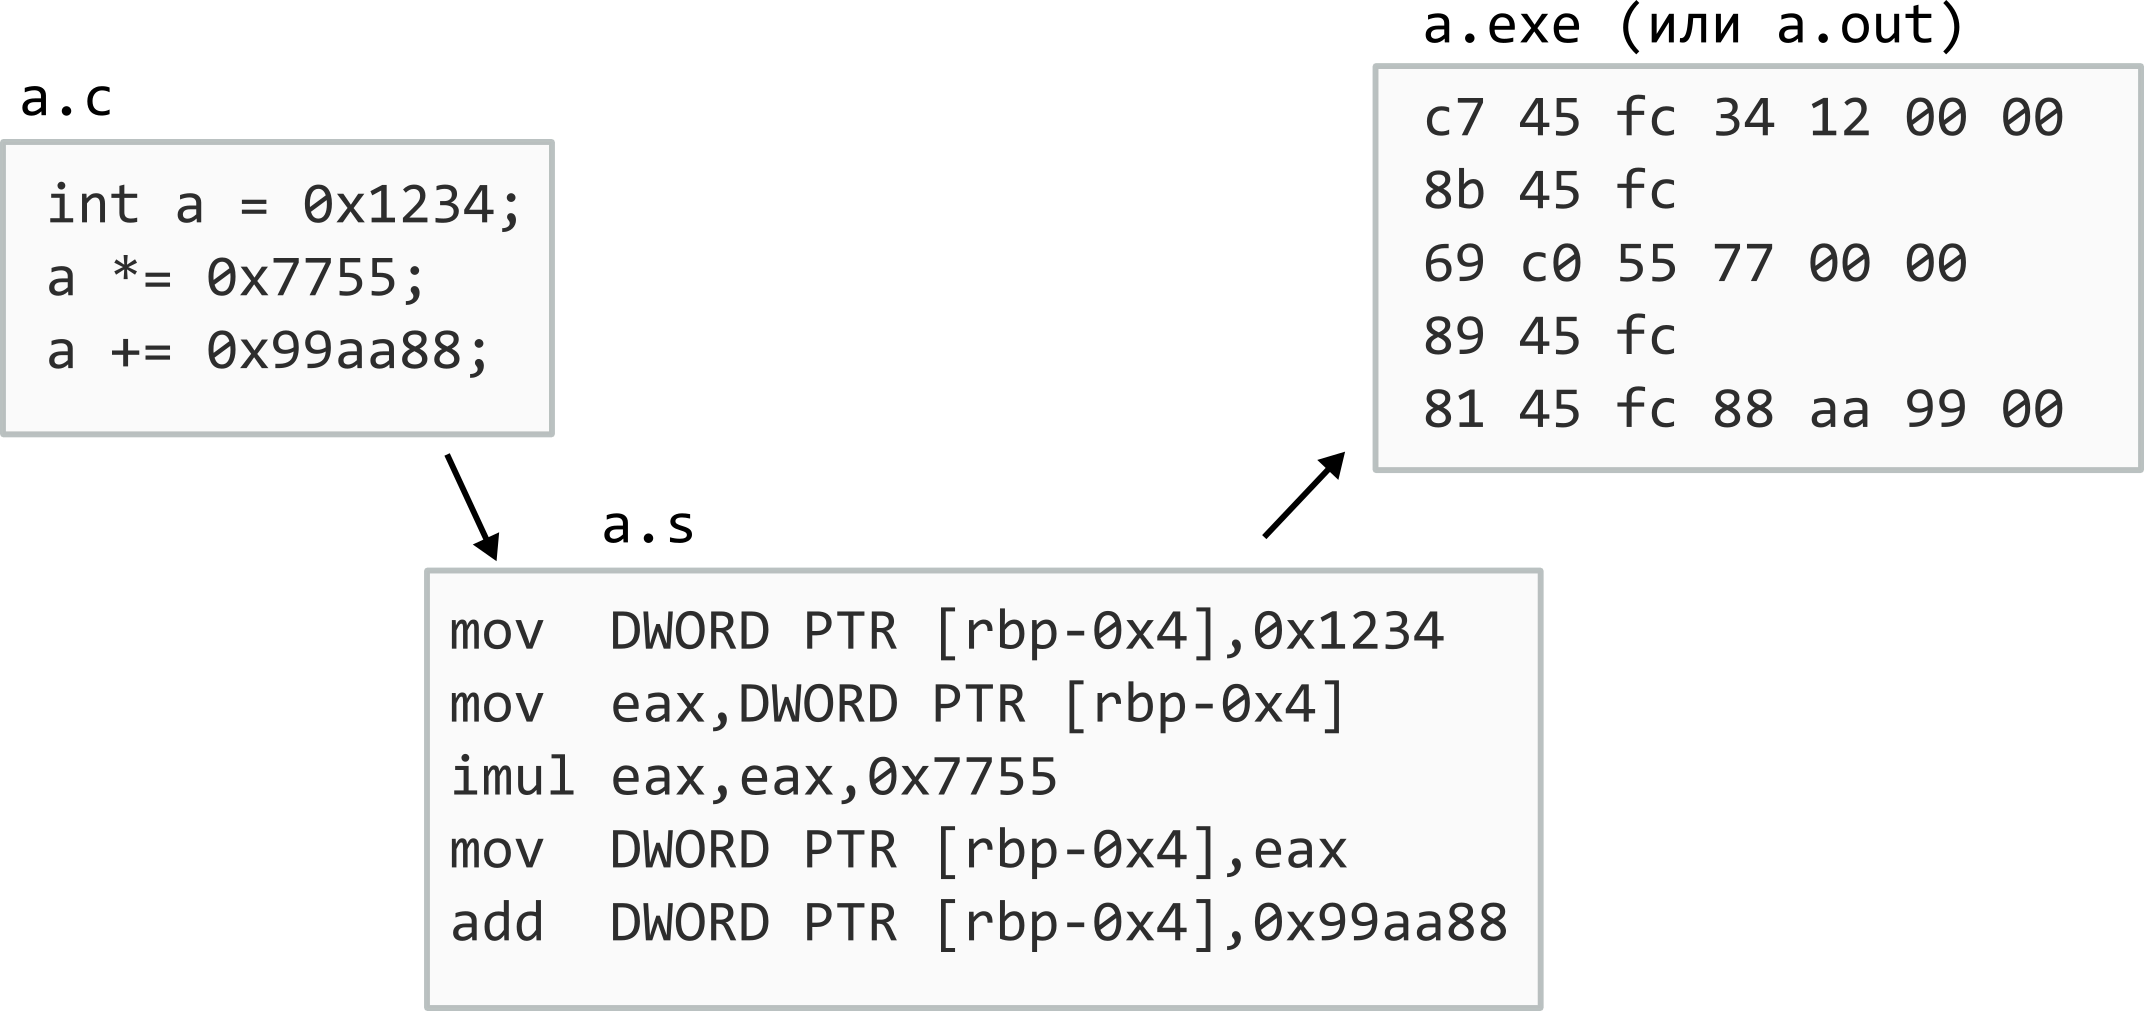
\includegraphics[scale=0.9]{../images/code_to_hex.png}
\end{center}
\subsubsection*{Из кода на C в код ассемблера:}
\begin{itemize}
\item Код на языке \texttt{C} (\texttt{a.c}) переводится в код на языке ассемблера (\texttt{a.s}). Эту операцию можно сделать командой
\begin{verbatim}
gcc -S -masm=intel ./a.c
\end{verbatim}
\item Регистры процессора -- это сверхбыстрая память, которая находится внутри процессора. Её размер очень мал(десятки байт), но процессор может доступиться к ней очень быстро (за 1 такт). В примере выше используются 2 регистра: \texttt{rbp} и \texttt{eax} (\texttt{eax} это часть регистра \texttt{rax}). 
\item Процессор может делать множество различных операций. Например, он может переместить некоторое количество байт из одного места в другое. Такие операции называются \texttt{mov}. Он может прибавить число (\texttt{add}) или умножить на целое (\texttt{imull}) и многое другое. \texttt{DWORD PTR} просто означает, что операция будет работать с 4-мя байтами.
\item В примере выше в регистре \texttt{rbp} содержится некоторый адрес. Квадратные скобочки означают разыменование. Поэтому строка
\begin{verbatim}
mov DWORD PTR [rbp-0x4],0x1234
\end{verbatim}
означает, что нужно положить число \texttt{0x1234} в 4 байта по адресу \texttt{rbp-0x4}
\item 
\begin{verbatim}
mov eax,DWORD PTR [rbp-0x4]
\end{verbatim}
означает, что нужно переместить 4 байта, которые хранятся по адресу \texttt{rbp-0x4} в регистр \texttt{eax}.
\item
\begin{verbatim}
imull eax,eax,0x7755
\end{verbatim}
означает, что нужно умножить содержимое \texttt{eax} на \texttt{0x7755} и сохранить результат в \texttt{eax}.
\item
\begin{verbatim}
mov  DWORD PTR [rbp-0x4],eax
\end{verbatim}
означает, что нужно переместить содержимое \texttt{eax} в память по адресу \texttt{rbp-0x4}.
\item
\begin{verbatim}
add  DWORD PTR [rbp-0x4],0x99aa88
\end{verbatim}
означает, что нужно добавить к числу по адресу \texttt{rbp-0x4} число \texttt{0x99aa88}.
\item В отличии от кода на языке \texttt{C}, код на языке ассемблера различаться на разных процессорах. Код с  вычислительной системы одной архитектуры скорей всего не будет работать на другой.
\end{itemize}
\subsubsection*{Из кода ассемблера в бинарный код (\texttt{.exe}):}
\begin{itemize}
\item Код на языке ассемблера (\texttt{a.s}) переводится в исполняемый файл. Эту операцию можно сделать командой \texttt{gcc a.s}
\item Каждая операция кодируется некоторым числом, называемым кодом операции (opcode).
\item Код операции \texttt{mov} на процессорах архитектуры \texttt{x86-64} может равняться \texttt{с7} или \texttt{8b} или \texttt{89} или некоторым другим  значениям(в зависимости от того куда и откуда мы копируем).
\item Например в строке:
\begin{verbatim}
c7 45 fc 34 12 00 00
\end{verbatim}
\begin{itemize}
\item \texttt{с7} означает, что это операция \texttt{mov} (присвоить число переменной в памяти)
\item \texttt{45} кодирует регистр \texttt{rbp}
\item \texttt{fc} кодирует смещение \texttt{-0x4}
\item \texttt{34 12 00 00} -- это 4-х байтовое число \texttt{0x1234} (порядок байт -- Little Endian)
\end{itemize}

\item
\begin{verbatim}
8b 45 fc
\end{verbatim}
\begin{itemize}
\item \texttt{8b} означает, что это операция \texttt{mov} (записать число, хранящееся в памяти, в \texttt{eax})
\item \texttt{45} кодирует регистр \texttt{rbp}
\item \texttt{fc} кодирует смещение \texttt{-0x4}
\end{itemize}

\item Все коды можно посмотреть тут \href{http://ref.x86asm.net/coder64.html}{ref.x86asm.net/coder64.html}
\item Получается, что в результате компиляции программы код превращается в последовательность байт (инструкций процессора). Эта последовательность байт и хранится в сегменте Текст.
\item А указатель на функцию является просто номером первого байта, с которого начинается функция в этом сегменте.
\item Менять сегмент Текст во время выполнения программы в большинстве современных операционных систем нельзя. 
\end{itemize}






\end{document}